%% LaTeX2e class for student theses
%% sections/content.tex
%%
%% Karlsruhe University of Applied Sciences
%% Faculty of  Computer Science and Business Information Systems
%% Distributed Systems (vsys)
%%
%% Prof. Dr. Christian Zirpins
%% christian.zirpins@hs-karlsruhe.de
%%
%%
%% Version 0.2, 2017-11-15
%%
%% --------------------------------------------------------
%% | Derived from sdqthesis by Erik Burger burger@kit.edu |
%% --------------------------------------------------------

\chapter{
	\iflanguage{english}{Basics for the secure implementation of decentralised social networks}{Grundlagen zur sicheren Umsetzung dezentraler sozialer Netzwerke}
}
\label{ch:fundamentals}
	\iflanguage{english}{
		This chapter gives an overview of general basics of social networks. It roughly explains what social networks are meant for, highlights the difference between centralized and decentralized social networks, and discusses security aspects.\\
		A cryptography subchapter is then introduced in which the procedures required for secure implementation are explained. It starts with a short introduction to cryptography and then briefly the \gls{rsa} procedure and a general description of signature algorithms.\\ 
		Finally the ActivityPub standard is introduced and classified, components of the protocol are described, the functionality of the client-to-server as well as server-to-server communication and associated standards are briefly explained.
		
	}{
		\todo{Allgemeine Grundlagen zu Sozialen Netzwerken/Social Media und deren Sicherheitsaspekte}
		\todo{Welche Klassen von Anwendungen und Implementierungen gibt es allgemein bei sozialen Netzwerken? Einordnen von ActivityPub!!}
		%\todo{AP Beschreibung in hinteren Teil des Grundlagenkapitels oder zu Beginn des 3. Kapitels}
		%Klassen von Anwendungen sowie Implementierungen erläutert.
		Dieses Kapitel gibt einen Überblick über allgemeine Grundlagen von sozialen Netzwerken. Es wird grob erläutert für was soziale Netzwerke gedacht sind; Der Unterschied zwischen zentralen, verteilen, dezentralen und förderierten sozialen Netzwerken herausgestellt sowie auf Sicherheitsaspekte eingegangen.\\
		
		Im Anschluss wird ein Kryptographie Unterkapitel eingeführt in dem die benötigten Verfahren für die sichere Umsetzung erläutert werden. Begonnen wird mit einer kurzen Einführung in Kryptographie. Darauf folgend wird kurz das RSA Verfahren sowie eine allgemeine Beschreibung von Signatur Algorithmen vorgenommen. HTTP Signaturen werden etwas ausführlicher beschrieben, da diese bei der Implementierung des Prototypen verwendet wurden.\\ 
		
		Darauf folgend wird der ActivityPub Standard eingeführt sowie eingeordnet, Bestandteile des Protokolls beschrieben, die Funktionsweise der Client-zu-Server sowie Server-zu-Server Kommunikation und zugehörige Standards kurz erläutert. Desweiteren wird auf die Authentifizierung und Datenintegrität bei ActivityPub eingegangen um damit folgende Fragen zu klären:
		\begin{itemize}
			\item Wie authentifiziert sich ein Benutzer gegenüber dem Server?
			\item Wie stellt man sicher, dass die Übertragenen Daten unverändert angekommen sind?
		\end{itemize}
	}
	\section{
		\iflanguage{english}{General principles of social networks}{Allgemeine Grundlagen sozialer Netzwerke}		
	}
	
		\subsection{
			\iflanguage{english}{Difference between centralised and decentralised social networks}{Unterschied zentraler zu dezentralen sozialen Netzwerken}
		}
		\subsection{
			\iflanguage{english}{Security aspects of social networks}{Sicherheitsaspekte sozialer Netzwerke}
		}
	\section{
		\iflanguage{english}{cryptography}{Kryptographie}
	}
	\iflanguage{english}{
		\glqq The term cryptography refers to the science of secret writing\grqq.\footnote{Dietmar Wätjen, 2018, p.1} One speaks of symmetric encryption when a message is encrypted in plain text by the sender with a secret key known to both parties and decrypted by the recipient with the same key.\footnote{Cf. Dietmar Wätjen, 2018, p.1}\\
		\begin{figure}[h]
			\begin{minipage}{\textwidth}
				\centering
				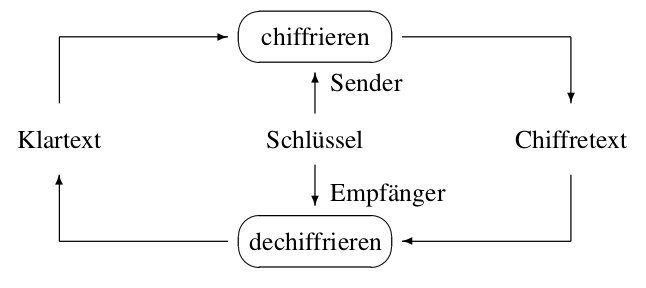
\includegraphics[scale=0.5]{figures/ver-und-entschluesseln.png}
				\quelle{(Wätjen, 2018, S.1)}
				\label{ver-und-entschluesselung}
				\caption{Symmetric en- and decryption}
			\end{minipage}
		\end{figure}
		\subsection{RSA}
		Asymmetric encryption is the term used when, instead of having a common key that has to be exchanged in advance, the participants each have a pair of keys (public and private keys). The \gls{rsa} method is one such asymmetric encryption method developed by the three mathematicians named after it in 1977. The \gls{rsa} method is probably the most commonly used public-key cryptosystem.\\
		
		\textbf{Example 1.} The interlocutors Alice and Bob, who both have a key pair, communicate with each other. Alice encrypts a message text with Bob's public key and sends the encrypted message to Bob. The latter in turn can decrypt the message with his private key.\footnote{Cf. Dietmar Wätjen, 2018, p.73 f.}\\
		\subsection{Signatures}
		So-called signatures can be used to ensure authenticity. The procedure briefly described above can not only be used to encrypt and decrypt messages, but also to sign them.\\
		Instead of the public key, the private key is used to generate a signature, in this case. This can then be verified with the public key of the corresponding private key.\\
		
		\textbf{Example 2.} Bob wants to send a message to Alice and make sure it hasn't been changed along the way. He uses his private key and applies it to a message to generate a signature. Both he transmits to Alice. Bob's public key can be used to verify that the message has been transmitted correctly.
	}{
		\glqq Unter dem Begriff Kryptographie ist die Wissenschaft vom geheimen Schreiben zu verstehen\grqq\footnote{Dietmar Wätjen, 2018, S.1}. Man spricht von symmetrischer Verschlüsselung wenn eine Nachricht im Klartext vom Sender mit einem geheimen Schlüssel, welcher beiden Parteien bekannt ist, verschlüsselt und vom Empfänger, mit demselben Schlüssel, entschlüsselt wird\footnote{Vgl. Dietmar Wätjen, 2018, S.1}.\\
		\begin{figure}[h]
			\begin{minipage}{\textwidth}
				\centering
				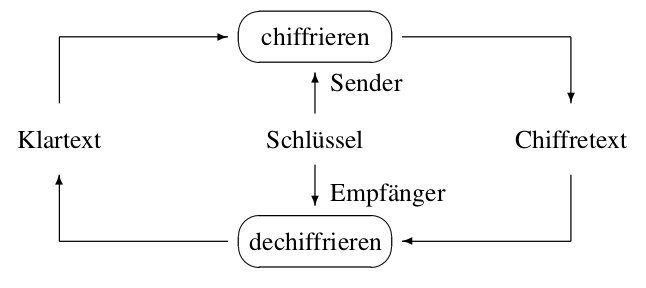
\includegraphics[scale=0.5]{figures/ver-und-entschluesseln.png}
				\quelle{(Wätjen, 2018, S.1)}
				\label{ver-und-entschluesselung}
				\caption{Symmetrische Ver- und Entschlüsselung}
			\end{minipage}
		\end{figure}\\
		Von asymmetrischer Verschlüsselung ist die Rede, wenn die Teilnehmer anstatt einen gemeinsamen Schlüssel zu haben, der im vor hinein ausgetauscht werden muss, jeder ein Schlüsselpaar, bestehend aus öffentlichem und privatem Schlüssel, besitzt.\\
		
		\subsection{RSA}
		Das \gls{rsa} Verfahren ist ein solches asymmetrisches Verschlüsselungsverfahren welches von den drei namens gebenden Mathematikern 1977 entwickelt wurde. Das \gls{rsa} Verfahren ist wohl das am häufigsten verwendete Public-Key-Kryptosystem.\\
		
		\textbf{Beispiel 1.} Die Gesprächspartner Alice und Bob, welche beide ein Schlüsselpaar besitzen, miteinander kommunizieren. Alice verschlüsselt einen Nachrichtentext mit dem öffentlichen Schlüssel von Bob und sendet die verschlüsselte Nachricht an Bob. Dieser kann seinerseits mit seinem privaten Schlüssel die Nachricht entschlüsseln\footnote{Vgl. Dietmar Wätjen, 2018, S.73 f.}.\\

		\subsection{Signaturen}
		Für die Sicherstellung der Authentizität können sogenannte Signaturen verwendet werden. Das oben kurz erläuterte \gls{rsa} Verfahren kann nicht nur zum Ver- und Entschlüsseln von Nachrichten benutzt werden, sondern auch zum signieren.\\
		Dabei wird statt des öffentlichen Schlüssels, der private Schlüssel benutzt um eine Signatur zu erzeugen. Diese kann dann mit dem öffentlichen Schlüssel des zugehörigen privaten Schlüssels verifiziert werden.\\
		
		Ein zugehöriges Beispiel wäre das folgende:\\
		\textbf{Beispiel 2.} Bob möchte eine Nachricht an Alice schicken und sichergehen, dass diese auf dem Weg nicht verändert wurde. Er verwendet seinen privaten Schlüssel und wendet diesen auf eine Nachricht an um eine Signatur zu erzeugen. Beides übermittelt er an Alice. Mit dem öffentlichen Schlüssel von Bob kann die fehlerfreie Übertragung der Nachricht verifiziert werden.\\
		
		\subsection{HTTP Signaturen}
		Eine \textit{HTTP Signatur} wird verwendet um die Authentizität sicherzustellen. Diese wird als Wert einer \glqq Signature\grqq~Kopfzeile eingetragen und besteht aus mehreren Teilen:
		\begin{itemize}}
			\item \textit{\textbf{keyId}}=keyId="https://example.org/activitypub/users/lea#main-key"
			\item \textit{\textbf{algorithm}}="rsa-md4"
			\item \textit{\textbf{headers}}="(request-target) date host content-type"
			\item \textit{\textbf{signature}}="DHeEH0Okmtf1ec/lbM1/F5FiLVfQfbWuoFf9t/TzNZiZ7ak"
		\end{itemize}
		Über die \textit{keyId}, was eine Referenz auf einen Schlüssel darstellt, kann der öffentliche Schlüssel angefragt werden. Dies wird beim verifizieren einer Signatur benötigt um die Übertragenen Daten auf ihre Authentizität hin zu prüfen.\\
		
		Welcher Hashing-Algorithmus bei der Erstellung verwendet wurde, kann über das \textit{algorithm} Feld der Signatur nachgeschlagen werden. Zudem muss der Algorithmus bei Erstellung in dieses Feld zum Nachschlagen eingetragen werden.\\
		
		Um die eigentliche Signatur zu erzeugen werden die in \textit{headers} angegebenen Kopfzeilen der HTTP Anfrage verwendet. Somit kann eingeschränkt werden welche Metadaten in die Signierung einfließen.\\
		
		Die bei der Signierung mit gegebenem Hashing-Algorithmus und Kopfzeilen erzeugte Signatur wird in das \textit{signature} Feld der HTTP Signatur eingetragen sowie die HTTP Signatur an sich als \glqq Signature\grqq~Kopfzeile der HTTP Anfrage gesetzt.\cite{http-signature}\\
	}
			
	\section{ActivityPub Standard}
	\iflanguage{english}{
		The ActivityPub Standard was developed on 23 January 2018 by the \gls{w3c} recommended\cite{activityPub} and by a working group of the \gls{w3c}, the \gls{swwg}\cite{socialWg,pushSocialWeb}. This group was active from July 21, 2014 until February 13, 2018\cite{socialWg} and developed ActivityPub, \gls{asc}\cite{activityStreamsCore} and \gls{asv}\cite{activityStreamsVocabulary} among others. The \gls{swwg} was a working group of the \gls{w3c} with the aim to define new protocols, vocabularies and \gls{api}'s for the access to social content of the so-called \gls{owp}\cite{social-wg-charter}.\\
		
		ActivityPub defines two protocol layers, as well as concepts, collections and interactions for decentralized social networks. A protocol layer is the client-to-server protocol (Social API) used to allow clients to access a server and receive requests from the client\cite{activityPub}.\\ 
		
		The second protocol layer consists of the promoted server-to-server protocol (Federation Protocol), which allows the individual instances of decentralized social networks to exchange content with each other. ActivityPub is based on already existing recommendations of the \gls{w3c}, which were partly also developed by the \gls{swwg} like e.g. \gls{asc} and \gls{asv}\cite{activityPub}.\\
		
		Other technologies such as \gls{JSON-LD} are also used to ensure extensibility. New ontologies and vocabularies can be used to add more syntactic definitions and semantic descriptions to the existing ones\cite{activityPub}. These vocabularies can be specified in the context of the \gls{JSON-LD} object. ActivityPub uses the \gls{AS2} vocabulary which is extended by \gls{asv}.
	}{
		Der ActivityPub Standard wurde am 23 Januar 2018 von der \gls{w3c} empfohlen\cite{activityPub} und von einer Arbeitsgruppe des \gls{w3c}, der \gls{swwg}\cite{socialWg,pushSocialWeb}, entwickelt. Diese Gruppe war vom 21. Juli 2014 bis zum 13 Februar 2018 aktiv\cite{socialWg} und entwickelte unter anderem ActivityPub, \gls{asc}\cite{activityStreamsCore} und \gls{asv}\cite{activityStreamsVocabulary}. Die \gls{swwg} war eine Arbeitsgruppe des \gls{w3c} mit dem Ziel neue Protokolle, Vokabulare und \gls{api}'s zu definieren für den Zugriff auf soziale Inhalte der sogenannten \gls{owp}\cite{social-wg-charter}.\\
		
		ActivityPub definiert zwei Protokollschichten, sowie Konzepte, Sammlungen und Interaktionen für dezentrale soziale Netzwerke. Eine Protokollschicht ist das Client-zu-Server Protokoll (Social API), um Clients den Zugriff auf die neusten an sie gesendeten Inhalte zu ermöglichen sowie zum entgegennehmen von Anfragen die vom Client abgesetzt wurden\cite{activityPub}.\\ 
		
		\begin{figure}[h]
			\begin{minipage}{\textwidth}
				\centering
				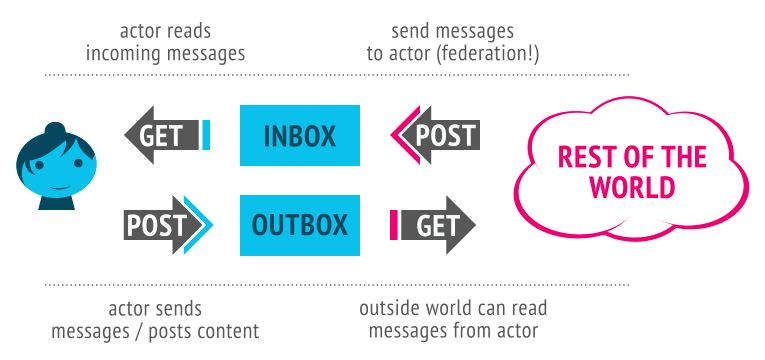
\includegraphics[scale=0.55]{figures/client-server-federated.png}
				\quelle{ActivityPub 2018 - Overview}
				\label{Client zu Server und Server zu Server Interaktionen}
				\caption{Schnittstellen des ActivityPub Protokolls}
			\end{minipage}
		\end{figure}
		
		Die zweite Protokollschicht besteht aus dem förderierten Server-zu-Server Protokoll (Federation Protocol), welches den einzelnen Instanzen von dezentralen sozialen Netzwerken den Austausch von Inhalten untereinander gestattet. ActivityPub setzt auf bereits bestehende Empfehlungen des \gls{w3c} auf, welche teilweise auch von der \gls{swwg} entwickelt wurden wie zB. \gls{asc} und \gls{asv}\cite{activityPub}. Die zwei Protokollschichten können unabhängig voneinander implementiert werden.\\
		
		Auch andere Technologien wie \gls{JSON-LD} werden genutzt um u. A. die Erweiterbarkeit zu gewährleisten. Über neue Ontologien und Vokabulare können weitere syntaktische Definitionen und semantische Beschreibungen zu den bestehenden hinzugefügt werden\cite{activityPub}. Diese Vokabulare können im Kontext des \gls{JSON-LD} Objektes, angegeben werden. Bei ActivityPub wird das \gls{AS2} Vokabular verwendet welches durch \gls{asv} erweitert wird.
	}
	\subsection{
		\iflanguage{english}{Elements of the protocol}{Bestandteile des Protokolls}
	}
	\iflanguage{english}{
		The client-to-server and promoted server-to-server protocol can be implemented independently. The former consists of a client and server part.\\
		
		In ActivityPub users are represented as \glqq actuators\grqq(actors). These can be not only individuals, but also applications, organizations, groups and services\cite{activityStreamsCore}. Each actuator object must have a \glqq Inbox\grqq~and \glqq Outbox\grqq, which must be ordered collections, as well as an ID and a type\cite{activityPub}. The ID must be globally unique. This can be guaranteed by a domain and protocol related URI or IRI such as \glqq https://example.org/users/alice\grqq or \glqq https://example.org/users/alice/áŷýà/2\grqq.
		
		The type of an actuator (e. g. "type": "Create") can vary between the five mentioned above.
		\lstinputlisting{resources/mastodon-macu.json}
	}{	
		Die Hauptbestandteile des ActivityPub Standards sind die folgenden:
		\begin{itemize}
			\item Aktoren
			\item Objekte
			\item Sammlungen
			\item Aktivitäten
		\end{itemize}
		In ActivityPub werden Benutzer als \glqq Aktoren\grqq(actors) dargestellt. Diese können nicht nur Personen, sondern auch Applikationen, Organisationen, Gruppen und Services sein\cite{activityStreamsCore}. Jedes Aktoren Objekt muss eine \glqq Inbox\grqq~und \glqq Outbox\grqq, welche geordnete Sammlungen sein müssen, sowie eine ID und ein Typ besitzen\cite{activityPub}. Die ID muss global einzigartig sein. Dies kann garantiert werden durch eine Domänen und Protokoll bezogene URI oder IRI wie z. B. \glqq https://example.org/users/alice\grqq oder \glqq https://example.org/users/álìcê\grqq. Der Typ eines Aktor (z. B. "type": "Person") kann variieren zwischen den fünf oben genannten.
		\lstinputlisting{resources/mastodon-macu.json}
	}
	\subsection{
		\iflanguage{english}{Related standards and components}{Zugehörige Standards und Komponenten}
	}
	\iflanguage{english}{
		ActivityPub uses the ActivityStreams data syntax and vocabulary. In addition, another security vocabulary\footnote{An ontology that defines security aspects such as public keys, signatures, and more} can be used to have definitions for providing a public key, signatures, encrypted content, and more. On April 22, 2016, the \glqq W3C Community Group\grqq~ published a draft report. It defines new syntax and semantics to enable Internet-based applications to encrypt, decrypt, digitally sign and verify linked data. It also contains vocabulary for creating and managing a decentralized public key infrastructure over the Internet\cite{security-vocab-linked-data}. A use case is retrieving a user's public key, using its object actuators to verify a message sent by users.
		
		\gls{JSON-LD} is an extension of the JSON format to represent linked data. JSON itself is a format that is often used on the web to exchange data. In essence, \gls{AS2} are also \gls{JSON-LD} objects. The \gls{AS2} context defines different classes and properties, not all of which are used. Typical classes are \glqq Activity\grqq, \glqq Link\grqq~and \glqq OrderedCollection\grqq. An example \gls{AS2} object looks like this: 	
		\lstinputlisting[caption={Example \gls{AS2} Object}, label=listing::as2-object, language=Javascript]{resources/example-as2-object.json}
	}{
		ActivityPub benutzt die ActivityStreams Daten Syntax und das Vokabular. Zusätzlich kann ein weiteres Sicherheitsvokabular\footnote{Eine Ontologie die Sicherheitsaspekte definiert wie öffentliche Schlüssel, Signaturen u.v.m.} benutzt werden um Definitionen zum Bereitstellen eines öffentlichen Schlüssels, Signaturen sowie Verschlüsselten Inhalten u.v.m. zu haben. Am 22 April 2016 hat die \glqq W3C Community Group\grqq~ einen Entwurfsbericht herausgebracht. Durch diesen wird neue Syntax und Semantik definiert um Internet basierten Applikationen das Verschlüsseln, Entschlüsseln sowie digitale Signieren und Verifizieren von verlinkten Daten (Linked Data) zu ermöglichen. Es enthält auch Vokabeln für die Erstellung und Verwaltung einer dezentralen Public-Key-Infrastruktur über das Internet\cite{security-vocab-linked-data}. Ein Anwendungsfall ist das holen des öffentlichen Schlüssels eines Nutzers, über dessen Aktoren Objekt, um eine von Nutzer gesendete Nachricht zu verifizieren.\\
		
		\glqq \gls{AS2}\grqq~beinhaltet Modelle für Aktoren, Aktivitäten, Intransitiven Aktivitäten, Objekte, Links, Sammlungen, Natürliche Sprachwerte (Strings) und für Internationalisierung. Das Kernvokabular von \gls{AS2} wird durch \gls{asv} erweitert. Dazu gehören verschiedene Aktivitätstypen wie z.B. \glqq Accept\grqq,\glqq Add\grqq,\glqq Remove\grqq,\glqq Delete\grqq~und \glqq Create\grqq\footnote{\href{https://www.w3.org/TR/activitystreams-vocabulary/}{activity-types https://www.w3.org/TR/activitystreams-vocabulary/}}, um Aktorentypen wie \glqq Person\grqq, \glqq Application\grqq~und \glqq Group\grqq\footnote{\href{https://www.w3.org/TR/activitystreams-vocabulary/}{actor-types https://www.w3.org/TR/activitystreams-vocabulary/}} sowie um verschiedenste Objekttypen wie \glqq Article\grqq, \glqq Event\grqq, \glqq Note\grqq~und \glqq Relationship\grqq\footnote{\href{https://www.w3.org/TR/activitystreams-vocabulary/}{object-types https://www.w3.org/TR/activitystreams-vocabulary/}}.\\
		
		\gls{JSON-LD} ist eine Erweiterung des JSON Formates um verlinkte Daten zu Repräsentieren. JSON an sich, ist ein Format welches im Web häufig Anwendung findet um Daten auszutauschen. Im Kern sind \gls{AS2} auch \gls{JSON-LD} Objekte. Der \gls{AS2} Kontext definiert verschiedene Klassen und Eigenschaften, von denen nicht alle benutzt werden. Typische Klassen sind \glqq Activity\grqq, \glqq Link\grqq~und \glqq OrderedCollection\grqq. Ein Beispiel \gls{AS2} Objekt sieht wie folgt aus: 	
		\lstinputlisting[caption={Beispiel \gls{AS2} Objekt}, label=listing::as2-object, language=Javascript]{resources/example-as2-object.json}
	}
	\subsection{
		\iflanguage{english}{Authentication and data integrity}{Authentifizierung und Datenintegrität}
	}
	\iflanguage{english}{
		The standard does not define any mechanisms for authentication and for ensuring data integrity. However, there are \glqq Best Practices\grqq~ for the implementation of these requirements.\\
		
		On the one hand, client to server authentication uses \glqq OAuth 2.0\grqq~Tokens, on the other hand, on the server side, \glqq HTTP\grqq~ or \glqq Linked Data Signatures\grqq to ensure data integrity.\\
		
		\glqq Data integrity includes measures to ensure that proprietary data cannot be removed or altered by unauthorized persons during processing or transmission. It ensures the consistency, accuracy and trustworthiness of the data throughout its lifetime and ensures that the relevant data of a data stream can be reconstructed.\grqq\footnote{\cite{data-integrity}}
		
		If an object is not only to be sent from the client to the server, but also forwarded between servers, a procedure other than HTTP signatures is required to ensure data integrity. The \glqq Best Practices\grqq~ recommend for such cases \glqq Linked Data Signatures\grqq. The biggest difference between HTTP signatures and \glqq Linked Data Signatures\grqq~ is what data is used to create the signature. For HTTP signatures, these are the headers. With \glqq Linked Data Signatures\grqq~, the object itself, i.e. the payload of an HTTP request, can also be used for signing instead of just the headers.
	}{
		Für die Authentifizierung und zum sichern der Datenintegrität definiert der Standard keine Mechanismen. Es gibt allerdings \glqq Best Practices\grqq~für die Umsetzung dieser Anforderungen.\\
	
		Zum einen werden bei der Client-zu-Server Authentifizierung \glqq OAuth 2.0 Bearer Tokens\grqq~benutzt, zum anderen auf der Server Seite \glqq HTTP\grqq~oder \glqq Linked Data Signatures\grqq zur Sicherstellung der Datenintegrität.\\

		Bei\glqq OAuth 2.0 Bearer Tokens\grqq~handelt es sich um eine Methode um auf geschützte Ressourcen zugreifen zu können\cite{oauth2}. ActivityPub nutzt diese für jegliche Interaktionen mit dem Server.\\
		
		\glqq Die Datenintegrität umfasst Maßnahmen damit geschützte Daten während der Verarbeitung oder Übertragung nicht durch unautorisierte Personen entfernt oder verändert werden können. Sie stellt die Konsistenz, die Richtigkeit und Vertrauenswürdigkeit der Daten während deren gesamten Lebensdauer sicher und sorgt dafür, dass die relevanten Daten eines Datenstroms rekonstruierbar sind\grqq\cite{data-integrity}.\\
		
		Um sicherzustellen das HTTP Anfragen beim Transport nicht verändert wurden, können HTTP Signaturen verwendet werden. Diesen verwenden einen kryptografischen Algorithmus um aus ausgewählten Kopfzeilen einer HTTP Anfrage einen kryptischen Zeichenfolge zu generieren. Auf der Empfängerseite kann die Zeichenfolge mit mitgelieferten und auch nachschlagbaren Information verifiziert werden.\\
		
		Wenn ein Objekt nicht nur vom Client zum Server gesendet, sondern auch zwischen Servern untereinander weitergeleitet werden soll wird zum Sicherstellen der Datenintegrität ein anderes Verfahren benötigt als HTTP Signaturen. Die \glqq Best Practices\grqq~empfehlen für solche Fälle \glqq Linked Data Signatures\grqq. Der größte Unterschied zwischen HTTP Signaturen und \glqq Linked Data Signatures\grqq~besteht darin, welche Daten zum Erstellen der Signatur verwendet werden. Bei HTTP Signaturen sind es die Kopfzeilen. Mit \glqq Linked Data Signatures\grqq~kann auch das Objekt selbst, also der Payload einer HTTP Anfrage, anstatt nur die Kopfzeilen, zum signieren verwendet werden.	
	}
